\documentclass{article}
\usepackage[T1]{fontenc}
\usepackage{lmodern}
\usepackage{graphicx}
\usepackage{amsmath,amssymb}
\usepackage[a4paper,margin=2cm]{geometry}
\usepackage[absolute,overlay]{textpos}
\setlength{\TPHorizModule}{1mm}
\setlength{\TPVertModule}{1mm}
\usepackage[indonesian]{babel}
\usepackage{hyperref}
\setlength{\emergencystretch}{2em}
% unit: Halaman 19

\begin{document}

% === Halaman 19 (llm) ===

\section*{5. Chosen-ciphertext attack}

Penyerang dapat memilih cipherteks tertentu dan mendekripsinya dengan oracle yang bisa mendekripsi, dan menggunakan hasil dekripsi untuk memecahkan cipher atau menemukan kunci.

\[ C_1, P_1 = D_k(C_1), C_2, P_2 = D_k(P_2), \dots, C_i, P_i = D_k(C_i) \]

Deduksi: $k$ (yang mungkin diperlukan untuk mendekripsi pesan pada waktu yang akan datang).

\vspace{10mm}

\begin{center}
\color{red} \textbf{Chosen-Ciphertext Attack}
\end{center}

% deskripsi: Diagram alur Chosen-Ciphertext Attack yang melibatkan Alice, Eve, dan Bob, menunjukkan bagaimana Eve memilih ciphertext, mendapatkannya melalui Bob, dan menganalisis plaintext hasilnya.
% bbox normalisasi: [0.3200, 0.7300, 0.7800, 0.9600]
\begin{textblock*}{96.60mm}(67.20mm,216.81mm)
\noindent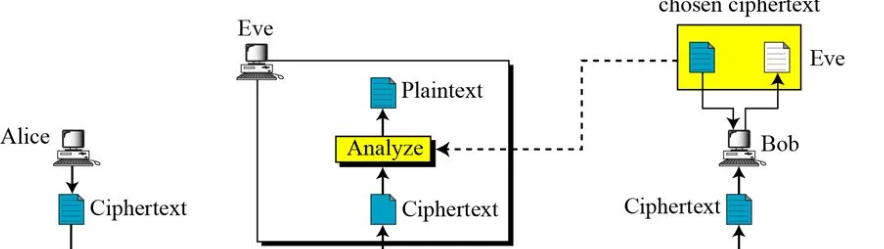
\includegraphics[width=96.60mm,height=68.31mm]{../../images/llm/page_019_img_01.png}%
\end{textblock*}

\end{document}
